%-----------------------------------------------------------------------
%
% Documentation for the Boundary and Interface Equation Solver
%
%-----------------------------------------------------------------------
\documentclass{article}
% \usepackage[bookmarks=true]{hyperref} 
\usepackage[bookmarks=true,colorlinks=true,linkcolor=blue]{hyperref}

% \input documentationPageSize.tex
\hbadness=10000 
\sloppy \hfuzz=30pt

% \voffset=-.25truein
% \hoffset=-1.25truein
% \setlength{\textwidth}{7in}      % page width
% \setlength{\textheight}{9.5in}    % page height

\usepackage{calc}
\usepackage[margin=1.in]{geometry}

%% \input homeHenshaw

\usepackage{amsmath}
\usepackage{amssymb}

\usepackage{verbatim}
\usepackage{moreverb}

\usepackage{graphics}    
\usepackage{epsfig}    
\usepackage{calc}
\usepackage{ifthen}
\usepackage{float}
% the next one cause the table of contents to disappear!
% * \usepackage{fancybox}

%\input{pstricks}\input{pst-node}
%\input{colours}

% define the clipFig commands:
% \input clipFig.tex
\usepackage{tikz}
% \input ../common/trimFig.tex

\newcommand{\bogus}[1]{}  % begin a section that will not be printed

% \newcommand{\ovFigures}{\homeHenshaw/OvertureFigures}
% \newcommand{\docFigures}{\homeHenshaw/OvertureFigures}
% \newcommand{\figures}{\homeHenshaw/res/OverBlown/docFigures}
% \newcommand{\obFigures}{\homeHenshaw/res/OverBlown/docFigures}  % note: local version for OverBlown

\newcommand{\Overture}{{\bf Overture\ }}
% \newcommand{\insDocDir}{\homeHenshaw/overtureFramework/cgDoc/ins}
\newcommand{\insDocDir}{.}

% -------------  -------------------
\newcommand{\bfss}{\sffamily\bfseries}


% *** See http://www.eng.cam.ac.uk/help/tpl/textprocessing/squeeze.html
% By default, LaTeX doesn't like to fill more than 0.7 of a text page with tables and graphics, nor does it like too many figures per page. This behaviour can be changed by placing lines like the following before \begin{document}

\renewcommand\floatpagefraction{.9}
\renewcommand\topfraction{.9}
\renewcommand\bottomfraction{.9}
\renewcommand\textfraction{.1}   
\setcounter{totalnumber}{50}
\setcounter{topnumber}{50}
\setcounter{bottomnumber}{50}


% -----definitions-----
\input ../common/wdhDefinitions.tex
% short for for begin{align} and \end{align}
\def\ba#1\ea{\begin{align}#1\end{align}}

% short for for begin{align*} and \end{align*}
\def\bas#1\eas{\begin{align*}#1\end{align*}}

% short for for begin{alignat}{3} and \end{alignat}
\def\bat#1\eat{\begin{alignat}{3}#1\end{alignat}}

% short for for begin{alignat*}{3} and \end{alignat*}
\def\bats#1\eats{\begin{alignat*}{3}#1\end{alignat*}}

\newcommand{\bse}{\begin{subequations}}
\newcommand{\ese}{\end{subequations}}

\newcommand{\p}{\partial}
\newcommand{\Ic}{\mathcal{I}}
\newcommand{\Jc}{\mathcal{J}}
\newcommand{\neqn}{{n_{\rm eq}}}
\newcommand{\nc}{n_{c}}
\newcommand{\Ig}{\Ic_g}
\newcommand{\Jg}{\Jc_g}
\newcommand{\eqn}{\text{eqn}}

% ***************************************************************************
\begin{document}



\vglue 5\baselineskip
\begin{flushleft}
{\Large
Documentation for the Boundary and Interface Equation Solver \\
}
\vspace{2\baselineskip}
William D. Henshaw,\\
Department of Mathematical Sciences, \\
Rensselaer Polytechnic Institute, \\
Troy, NY, USA, 12180.
% \footnote{This work was performed under the auspices of the U.S. Department of Energy (DOE) by
% Lawrence Livermore National Laboratory under Contract DE-AC52-07NA27344 and by 
% DOE contracts from the ASCR Applied Math Program.}  \\
% Centre for Applied Scientific Computing  \\
% Lawrence Livermore National Laboratory      \\
% Livermore, CA, 94551.  \\
% henshaw@llnl.gov \\
% http://www.llnl.gov/casc/people/henshaw \\
% http://www.llnl.gov/casc/Overture\\
\vspace{\baselineskip}
\today\\
% \vspace{\baselineskip}
% LLNL-SM-455851

\vspace{4\baselineskip}

\noindent{\bf Abstract:}
The BoundarySolver class can be used to solve the coupled equations that result from applying
boundary conditions (such as high-order accurate compatibility conditions) and interface conditions.
\end{flushleft}

% \clearpage
\tableofcontents
% \listoffigures

% \clearpage
\section{Introduction}

Consider solving the the heat equation or wave equation,
\ba
& \p_t^2 u = \Delta u , \qquad \xv\in\Omega,  \\
& \p_t u = \Delta u, \qquad \xv\in\Omega, 
\ea
with Dirichlet, Neumann or mixed boundary conditions,
\bat
&     u(\xv,t) = g^d(\xv), \qquad&& \xv \in \partial\Omega, \\
&   \alpha \p_n u(\xv,t)  + \beta u(\xv,t) = g^n(\xv), \qquad&& \xv \in \partial\Omega. 
\eat
A high-order difference approximation may use compatibility conditions as additional
numerical boundary conditions to determine values at the ghost points. These conditions may
couple the unknown ghost values along the boundary and require the solution to a system
of equations. The BoundarySolver class can be used to form and solve these equations.

\medskip
Consider the example of imposing the compatibility boundary condition
\ba
   \Delta u(\xv) = g(\xv) , \qquad \xv\in\partial\Omega.
\ea
to second-order accuracy as a means to evaluate the ghost point values. 
Let the discrete approximation be
\ba
   \Delta u_{ij} = g_j  , \qquad i=0.
\ea
On a curvlinear grid, cross terms will appear in the approximation for $\Delta_{h}$ and
the ghost points $u_{-1,j}$ will be coupled. To determine the ghost values, a system
of equations must be solved.


A fourth-order approximaton may use two compatibility conditions
\ba
  & \Delta_{4h} u_{ij} = g^1_{j}, \\
  & \Delta_{2h}^2 u_{ij} = g^2_{j} 
\ea
which couple the values at the two ghost points $u_{-1,j}$ and $u_{-2,j}$. Again, 
a system of equations must be solved to determine the values at the ghost points.

\medskip
More generally we may wish to solve a system of equations
\bas
   \p_t^2 \uv = \Delta \uv , \qquad \xv\in\Omega,  
\eas
where $\uv(\xv,t)$ has $\nc$ components. In this case the numerical boundary conditions
will couple the different components and these will all have to be solved as
a coupled system.

% -------------------------------------------------------------------------------------------
\section{Boundary conditions}

The BoundarySolver Class can be used to form and solve the discrete equations.
There are multiple ways to fomr the equations. 
In the simplest approach the user should supply a function that evaluates the
boundary conditions in a \textit{forward manner}
\begin{verbatim}
  int evalBC( realMappedGridFunction & u, RealArray & g, 
              Index & Ib1, Index & Ib2, Index & Ib3, RealArray & f )
\end{verbatim}
For example, this routine could evaluate
\ba
  & f(i_1,i_2,i_3,0) =  \Delta_{4h} u(i_1,i_2,i_3) - g(i_1,i_2,i_3,0), \\
  & f(i_1,i_2,i_3,1) =  \Delta_{2h}^2 u(i_1,i_2,i_3) - g(i_1,i_2,i_3,1)
\ea
at points $\iv=(i_1,i_2,i_3)$ on the boundary defined by \texttt{Ib1},\texttt{Ib2}, and \texttt{Ib3}.

The function \texttt{constructBoundaryConditionCoefficients} can then be used to form
the discrete equations that need to be solved. This is done by a discrete \textit{delta-function approach}.
The coefficients in the equations can be automatically found by evaluating the forward-equations
with a function $u(i_1,i_2,i_3)$ that is a value ``1'' at one ghost point and zero at all points. By repeatedly
evaluating the boundary conditions, the discrete matrix can be found (this process
is made more efficient by evaluating multiple coefficients at once). 


% -------------------------------------------------------------------------------------------
\section{Interface equations}

\newcommand{\Dc}{\mathcal{D}}
\newcommand{\Kc}{\mathcal{K}}
Interface conditions can also be solved using the BoundarySolver class.
Example interface conditions for a second-order accurate scheme might be the jump conditions
\ba
&   \Kc_1 \p_n u^1 - \Kc_2  \p_n u^2 = g^1 , \\ 
&   \Dc_1 \Delta u^1 - \Dc_2 \Delta u^2 = g^2.
\ea
where $u^1$ is the solution on one side of the interface and $u^2$ is the solution
on the other side.

As for the case of boundary conditions, the user may supply a function that evaluates the
interface equations in a forward manner, 
{\small
\begin{verbatim}
int evalInterface( 
   realMappedGridFunction & u1, Index & Ib1, Index & Ib2, Index & Ib3, int side, int axis,
   realMappedGridFunction & u2, Index & Jb1, Index & Jb2, Index & Jb3, int side2, int axis2,
   RealArray & g, RealArray & f )
\end{verbatim}
}%
and the function \texttt{constructInterfaceCoefficients} can be used to form the discrete
equations using the discrete delta-function approach.
                   
% -------------------------------------------------------------------------------------------
\section{Grid point index to sparse matrix numbering} % Discrete coefficients and the grid-function to sparse-matrix mapping}

\newcommand{\equationToIndex}{\text{equationToIndex}}
\newcommand{\indexToEquation}{\text{indexToEquation}}

The BoundarySolver class solves a sparse matrix equation of the form
\bas
         A \wv = \bv
\eas
where the vector $\wv\in\Real^\neqn$ holds the $\neqn$ unknown ghost values arranged into a single vector. 
Each entry $w_k$ in $\wv$ corresponds to a ghost point on a grid function $u(i_1,i_2,i_3,n)$ and we need
to know this correspondence between $k$ and $(i_1,i_2,i_3,n)$. For interface problems, we also need to
know the grid number of the ghost point value. 


\bigskip
To build the sparse matrix of equations whose solution defines the ghost point values
we need to define the mapping (and its inverse) between the grid point index location (and component number)
of the ghost points 
\ba
(\iv,n), \qquad \iv\in\Ig, \quad n=0,1,\ldots,\nc-1, 
\ea
and the sparse matrix equation number
\ba
  \eqn=0,1,\ldots,\neqn-1.
\ea
Here $\iv\in\Ig$ denote the ghost points holding unknowns.
The mapping from equation ``$\eqn$'' to grid index is given by (using Matlab function notation)
\ba
    [ \iv,n,grid ] = \equationToIndex(\eqn)
\ea
The inverse mapping from grid index to equation number is
\ba
    [ \eqn ] = \indexToEquation(\iv,n,grid)
\ea

\newcommand{\labelSize}{\footnotesize}

The equation ordering is
arbitrary. A fairly natural choice is made so as to make the sparse matrix have non-zero entries along the diagonal in
typical situtations. 
Figure~\eqref{fig:equationNumbering} shows some example equation numbering for the ordering we have chosen.
The equations are numbered with ghost point 1 followed by ghost point 2, etc, and with the 
equations then following the ordering of the boundary points. 
\begin{figure}[hbt]
\begin{center}
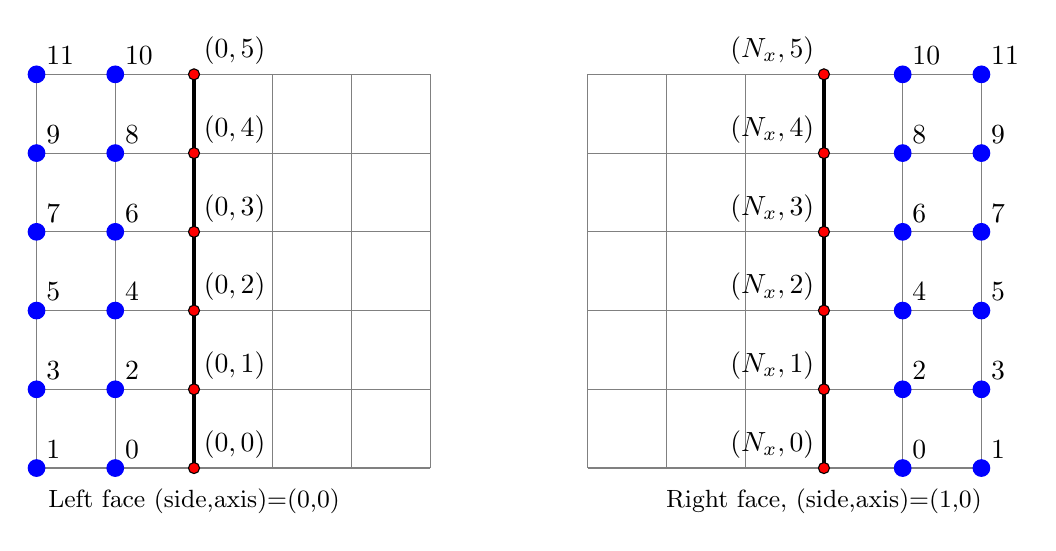
\begin{tikzpicture}
% 
  \draw[gray] (-2,0) grid (3,5);
% -----
  \draw[very thick] (0,0) -- (0,5);  
  %
  \foreach \x/\y in {0/0,0/1,0/2,0/3,0/4,0/5} {
    \draw (\x,\y) node[anchor=south west] {\labelSize $(\x,\y)$ };
    \draw[black,fill=red] (\x,\y) circle (2pt);
  }
  %
  \foreach \y/\yy in {0/0,1/2,2/4,3/6,4/8,5/10} {
    \draw (-1,\y) node[anchor=south west] { \yy };
    % \node at (-1,\y) [circle,fill=black] {}; 
    \draw[blue,fill=blue] (-1,\y) circle (3pt);
  }
  %
  \foreach \y/\yy in {0/1,1/3,2/5,3/7,4/9,5/11} {
    \draw (-2,\y) node[anchor=south west] { \yy };
    % \node at (-1,\y) [circle,fill=black] {}; 
    \draw[blue,fill=blue] (-2,\y) circle (3pt);
  }
  \draw (0,0) node[anchor=north,yshift=-4pt] {\small Left face (side,axis)=(0,0)};
% -----
 \begin{scope}[xshift=8cm]
  \draw[gray] (-3,0) grid (2,5);
  \draw[very thick] (0,0) -- (0,5);  
  %
  \foreach \x/\y in {0/0,0/1,0/2,0/3,0/4,0/5} {
    \draw (\x,\y) node[anchor=south east] {\labelSize $(N_x,\y)$ };
    \draw[black,fill=red] (\x,\y) circle (2pt);
  }
  %
  \foreach \y/\yy in {0/0,1/2,2/4,3/6,4/8,5/10} {
    \draw (1,\y) node[anchor=south west] { \yy };
    % \node at (-1,\y) [circle,fill=black] {}; 
    \draw[blue,fill=blue] (1,\y) circle (3pt);
  }
  %
  \foreach \y/\yy in {0/1,1/3,2/5,3/7,4/9,5/11} {
    \draw (2,\y) node[anchor=south west] { \yy };
    % \node at (-1,\y) [circle,fill=black] {}; 
    \draw[blue,fill=blue] (2,\y) circle (3pt);
  }
  \draw (0,0) node[anchor=north,yshift=-4pt] {\small Right face, (side,axis)=(1,0)};
 \end{scope}
\end{tikzpicture}  
\end{center}
\caption{Example equation numbering for the ghost points on the left or right face of a grid.
   The boundary points are marked with red circles, the unknown ghost points with blue circles.}
\label{fig:equationNumbering}
\end{figure}

For the example in Figure~\eqref{fig:equationNumbering} for the left face, the some equation numbers
would map to grid index locations as (ignoring the component and grid numbers)
\bas
  &   [ \iv=(-1,0) ] = \equationToIndex(0), \\
  &   [ \iv=(-2,0) ] = \equationToIndex(1), \\
  &   [ \iv=(-1,1) ] = \equationToIndex(2), \\
  &   [ \iv=(-2,1) ] = \equationToIndex(3), 
\eas
while some grid index locations would map to equation numbers as 
\bas
&   [\eqn=2]=  \indexToEquation(\iv=(-1,1)), \\
&   [\eqn=5]=  \indexToEquation(\iv=(-2,2)), \\
&   [\eqn=8]=  \indexToEquation(\iv=(-1,4))
\eas

\newcommand{\beqn}{\text{beqn}}
The equation numbers are stored in an array of integers
\bas
      \beqn(i_1,i_2,i_3), \qquad \iv=(i_1,i_2,i_3) \in \Ig
\eas
For multiple solution components, the equation numbering is
\bas
    \indexToEquation(\iv,n) = n + \nc\, \beqn(i_1,i_2,i_3)
\eas
so that different components at a given grid point are adjacent to each other in $\wv$. 
For the example of the left face, the unknowns $u_{\iv,n}$ thus appear in the linear order
\bas
\wv = \left[
         u_{-1,0,0,n=0}, u_{-1,0,0,n=1}, ~
         u_{-2,0,0,n=0}, u_{-2,0,0,n=1}, ~
         u_{-1,1,0,n=0}, u_{-1,2,0,n=1}, \cdots
      \right]
\eas
with component $n=0$ followed by component $n=1$.

% --------------------------------------------------------
\clearpage
\section{Interfaces}

For an interface between two grids 
the equation numbering alternates between the
left and right sides as shown in Figure~\ref{fig:equationNumberingInterface}.
Note that, in general, the right side of the interface could be indexed differently than the left side; we
use $\iv\in\Ig$ to denote ghost points on the left side and $\jv\in\Jg$ to denote ghost points on the right side.
%
Given the basic boundary equation numbering for the left and right sides defined in the
previous section (i.e. assuming no interface)
\bats
    &  \beqn1(i_1,i_2,i_3), \qquad&& \iv=(i_1,i_2,i_3) \in \Ig, \\
    &  \beqn2(j_1,j_2,j_3), \qquad&& \jv=(j_1,j_2,j_3) \in \Jg, 
\eats
the equation number of the interface is then
\bas
\indexToEquation(\iv) =
    \begin{cases}
        2\, \beqn1(i_1,i_2,i_3),     \quad& \text{(left side)}, \\
        2\, \beqn2(i_1,i_2,i_3) +1 , \quad& \text{(right side)},
    \end{cases}
\eas

\begin{figure}[hbt]
\begin{center}
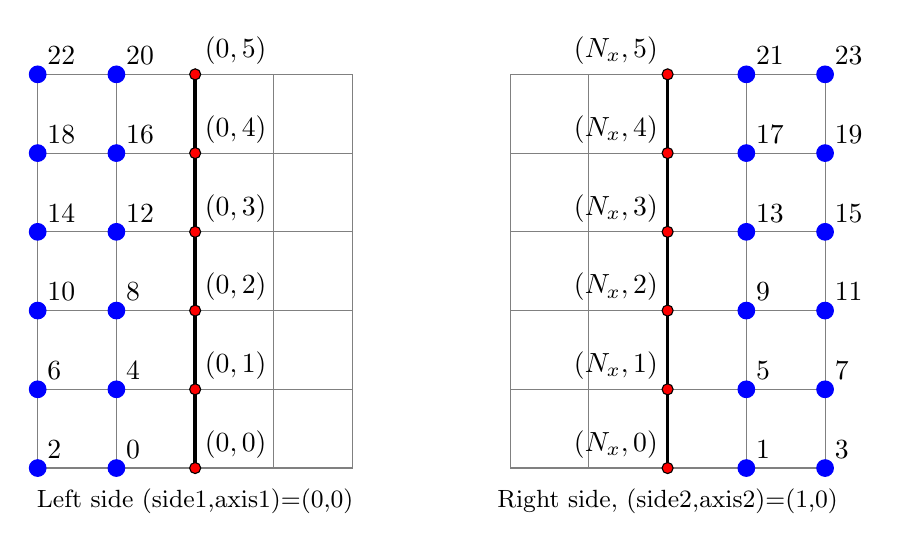
\begin{tikzpicture}
% 
  \draw[gray] (-2,0) grid (2,5);
% -----
  \draw[very thick] (0,0) -- (0,5);  
  %
  \foreach \x/\y in {0/0,0/1,0/2,0/3,0/4,0/5} {
    \draw (\x,\y) node[anchor=south west] {\labelSize $(\x,\y)$ };
    \draw[black,fill=red] (\x,\y) circle (2pt);
  }
  %
  \foreach \y/\yy in {0/0,1/4,2/8,3/12,4/16,5/20} {
    \draw (-1,\y) node[anchor=south west] { \yy };
    % \node at (-1,\y) [circle,fill=black] {}; 
    \draw[blue,fill=blue] (-1,\y) circle (3pt);
  }
  %
  \foreach \y/\yy in {0/2,1/6,2/10,3/14,4/18,5/22} {
    \draw (-2,\y) node[anchor=south west] { \yy };
    % \node at (-1,\y) [circle,fill=black] {}; 
    \draw[blue,fill=blue] (-2,\y) circle (3pt);
  }
  \draw (0,0) node[anchor=north,yshift=-4pt] {\small Left side (side1,axis1)=(0,0)};
% -----
 \begin{scope}[xshift=6cm]
  \draw[gray] (-2,0) grid (2,5);
  \draw[very thick] (0,0) -- (0,5);  
  %
  \foreach \x/\y in {0/0,0/1,0/2,0/3,0/4,0/5} {
    \draw (\x,\y) node[anchor=south east] {\labelSize $(N_x,\y)$ };
    \draw[black,fill=red] (\x,\y) circle (2pt);
  }
  %
  \foreach \y/\yy in {0/1,1/5,2/9,3/13,4/17,5/21} {
    \draw (1,\y) node[anchor=south west] { \yy };
    % \node at (-1,\y) [circle,fill=black] {}; 
    \draw[blue,fill=blue] (1,\y) circle (3pt);
  }
  %
  \foreach \y/\yy in {0/3,1/7,2/11,3/15,4/19,5/23} {
    \draw (2,\y) node[anchor=south west] { \yy };
    % \node at (-1,\y) [circle,fill=black] {}; 
    \draw[blue,fill=blue] (2,\y) circle (3pt);
  }
  \draw (0,0) node[anchor=north,yshift=-4pt] {\small Right side, (side2,axis2)=(1,0)};
 \end{scope}
\end{tikzpicture}  
\end{center}
\caption{Interface between two grids: the equation numbering alternates from the left side of the interface
         to the right side.
   The boundary points are marked with red circles, the unknown ghost points with blue circles.}
\label{fig:equationNumberingInterface}
\end{figure}


When there are multiple components the equation numbering alternates between the left and right sides
\bas
\indexToEquation(\iv,n) =
    \begin{cases}
       2\, \Big( n +  \nc\, \beqn1(i_1,i_2,i_3)\Big),     \quad& \text{(left side)}, \\
       2\, \Big( n +  \nc\, \beqn2(i_1,i_2,i_3)\Big) +1 , \quad& \text{(right side)},
    \end{cases}
\eas

% ------------------------------------------------------------------------------------
% \clearpage
\section{Reordering equations}

Some sparse solvers do not pivot and may require non-zero diagonal entries in the sparse matrix.
Currently reordering is needed for interface equations with multiple ghost points and multiple
components. 

The BoundarySolver class includes the capability to reorder the
associated with
a given grid point using a \texttt{rowPermutation} array.
At each boundary point there are
\bas
   n_e = n_g \, n_c, \quad \text{(number of equations at each boundary point)}
\eas
equations where $n_g$ is the number of ghost points and $n_c$ is the number of components. 
At each interface point there are twice as many equations
\bas
   n_e = 2 \, n_g \, n_c,  \quad \text{(number of equations at each interface point)}
\eas
The default ordering of equations, denoted by $m=0,1,\ldots,n_e-1$
is defined by the order of equations in the
user supplied function \texttt{evalBc} or \texttt{evalInterface}. 
The new ordering is defined through a permutation of $\{ 0,1,2,\ldots,n_e-1\}$ and stored in the array
\ba
     \tilde{m} = \texttt{rowPermutation}(m) .
\ea
The inverse of this permutation is also needed and stored in the \texttt{inverseRowPermutation} array.

\end{document}


% ----------------------------------------------------------------------------------------------------------



